\documentclass[14pt]{extarticle}
% math symbols
\usepackage{sfg}


\usepackage{amssymb,amsmath}
\synctex=1
% for different compilers
\usepackage{ifpdf}
% geometry of page
\usepackage[margin=2cm]{geometry}

% if pdflatex, then
\ifpdf
\usepackage[russian]{babel}
\usepackage[utf8]{inputenc}
\usepackage[unicode]{hyperref}
\usepackage[pdftex]{graphicx}
\usepackage{cmlgc}
% if xelatex, then
\else
% math fonts
\usepackage{fouriernc}
% xelatex specific packages
\usepackage[xetex]{hyperref}
\usepackage{xltxtra}	% \XeLaTeX macro
\usepackage{xunicode}	% some extra unicode support
\defaultfontfeatures{Mapping=tex-text}
\usepackage{polyglossia}	% instead of babel in xelatex
\usepackage{indentfirst}	% 
\setdefaultlanguage{russian}
% fonts
\newfontfamily\cyrillicfont{SchoolBookC}
\newfontfamily\cyrillicfontsf{TextBookC}
\setmonofont{Consolas}
\fi

% several pictures in one figure
\usepackage{subfig}
% calc in TeX expressions
\usepackage{calc}
% nice pictures and plots
\usepackage{pgfplots,tikz,circuitikz}
% different libraries for pictures
\usetikzlibrary{%
  arrows,%
  calc,%
  patterns,%
  decorations.pathreplacing,%
  decorations.pathmorphing,%
  decorations.markings,%
  intersections,%
  decorations.text%
}

\usepackage{tkz-euclide}

\usepackage{enumitem}
\renewcommand{\theenumi}{(\asbuk{enumi})}
\renewcommand{\labelenumi}{\asbuk{enumi})}
\AddEnumerateCounter{\Asbuk}{\@Asbuk}{\CYRM}
\AddEnumerateCounter{\asbuk}{\@asbuk}{\cyrm}

\begin{document}

\section*{Задача}

\subsection*{Условие}
Пусть $ABCDA_1B_1C_1D_1$ -- Куб. Нарисуйте прямую, которая проходит:

\begin{enumerate}

\item Через Точку $C$ и перпендикулярна $(C_1D_1)$;

\item Через точку $C_1$ и Перпендикулярна $(BD)$

\item Через точку $B_1$ и Перпендикулярна $(AC)$

\item Через точку $B$ и Перпендикулярна $(B_1D)$.

\end{enumerate}
\subsection*{Решение}
\begin{enumerate}

\item Это $CC_1$ -- ребро куба.

\item Это $C_1O$, где O -- центр основания $ABCD$. медиана равнобедренного треугольника $\Delta BC_1D$.

\item Это $B_1O$ -- медиана равнобедренного треугольника $\Delta AB_1C$.

\item Это $BM$ (см. рисунок).

\end{enumerate}

\vspace{0.5 cm}

 Найдем положение точки $M$. Для этого Заметим, что $\Delta BB_1D$ и $\Delta MB_1B$ подобны по двум углам. А значит

\begin{equation}
	\frac{BD}{B_1B} = \frac{B_1M}{B_1B}.
\end{equation}

Как следствие

\begin{equation}
	B_1M = \frac{{B_1B}^2}{B_1D}.
\end{equation}

Из теоремы Пифагора мы знаем, что $B_1D = \sqrt{3} B_1B$. В результате

\begin{equation}
	B_1M = \frac{{B_1B}^2}{B_1D} = \frac{{B_1D}^2}{3B_1D} = \frac{B_1D}{3}.
\end{equation}
\newpage
\begin{figure}[h]
	\centering
	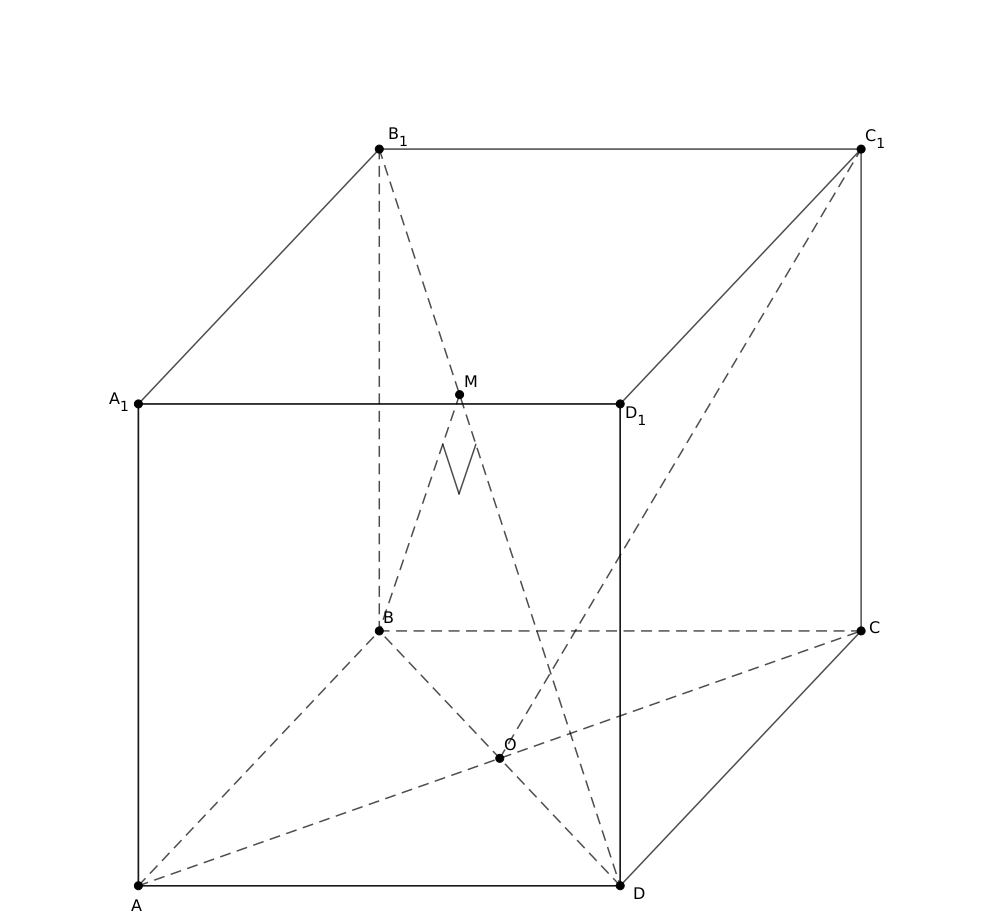
\includegraphics[width=1\textwidth]{{/home/galqiwi/geoma/5.3}.png}
\end{figure}


\end{document}